\mode<presentation>
{
    \usetheme{Relax}
    \defbeamertemplate{footline}{Empty}{}
    \setbeamersize{text margin left=8mm,text margin right=8mm}
    %\setbeamerfont{section title}{size=\Huge}
    \defbeamertemplate*{section page}{Iceland}[3][]
    {
        \begin{tikzpicture}[overlay,remember picture]
            \usebeamercolor{section page background canvas}
            \fill[bg] (current page.south west) rectangle (current page.north east);
            \node[anchor=west] (photo) at ($(current page.west)+(5mm,0)$) {\includegraphics[width=0.85\textwidth]{#2}};
            \node[text depth=0.5ex, below = 3mm of photo.south east, anchor=east]{#3};
            \node[text depth=0.5ex, above = 4mm of photo.north west, anchor=west]
                  {\usebeamerfont{section title}\usebeamercolor[fg]{section title}\insertsectionhead};
            \node[anchor=north east, inner sep=0] (plan) at ($(current page.north east)-(1mm,1mm)$) {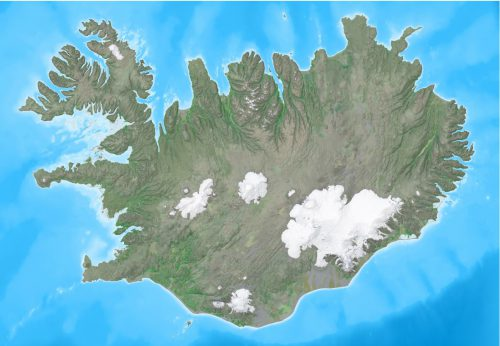
\includegraphics[width=0.2\textwidth, clip, trim=0 0 0 1mm]{Map}};
            \ifthenelse{\isempty{#1}}{}%
            {
                \begin{scope}[x={($ (plan.south east) - (plan.south west) $ )},y={( $ (plan.north west) - (plan.south west)$ )}, shift={(plan.south west)}]
                    %\draw[help lines,xstep=.1,ystep=.1] (0,0) grid (1,1);
                    \node[anchor=south, inner sep=0] at (#1) {
\includegraphics[width=2mm]{Pin}};
                \end{scope}
            }
        \end{tikzpicture}
    }
}

\AtBeginSection[] % <- Empty optional argument, do nothing for \section*
{
    \begin{frame}[plain, noframenumbering]{}
         \sectionpage
    \end{frame}
}

%===============================================================%
\title{Introduction to Bash scripting language}
\author{Alessandro Sciarra}
\institute{Z02~--~Software Development Center}
\titlegraphic{
\includegraphics[width=25mm]{LogoCRC}}
\titlepagelogo{
\includegraphics[width=25mm]{LogoGoethe}}
%===============================================================%
